\documentclass{article}
\usepackage{bm}
\usepackage{url}
\usepackage{cite}
\usepackage{tikz}
\usepackage{ulem}
\usepackage{float}
\usepackage{array}
\usepackage{framed}
\usepackage{amsthm}
\usepackage{hhline}
\usepackage{balance}
\usepackage{amssymb}
\usepackage{amsmath}
\usepackage{amsmath}
\usepackage{courier}
\usepackage{booktabs}
\usepackage{verbatim}
\usepackage{graphicx}
\usepackage{subfigure}
\usepackage{enumerate}
\usepackage{algorithm}
\usepackage{pseudocode}
\usepackage{algpseudocode}
\usepackage{soul,xcolor}
\usepackage{yfonts,color}
\usepackage{epsfig,epstopdf}
\title{Learning based Cognitive Radio Access via Randomized Point-based Approximate POMDPs\\\Large{IEEE TCCN 2021: Addressing Reviewer Comments}}
\author{Bharath Keshavamurthy and Nicol\`{o} Michelusi}
\date{April 2021}
\begin{document}
\maketitle
\section{Addressing Reviewer-1 Comments}

\begin{enumerate}

    \item \textbf{Comment}: As claimed, PUs typically occupy a set of adjacent channels, which leads to frequency correlation.  That is, the occupancy of frequency band $k$ is related to the occupancy of the adjacent frequency bands $k{-}1$ and $k{+}1$. However, the authors assume that the occupancy of frequency band k only depends on the occupancy of frequency band  $k{-}1$ in Eq. $(6)$. Is that reasonable?\\
    \textbf{Addressal}: Although we make a claim in our original manuscript that the Markov chain across frequency is reversible (``If the frequency correlation direction is changed, i.e., the occupancy of channel $k{+}1$ influences the occupancy of channel $k$ (bottom-up vs top-down correlation), our model and subsequent analyses still hold"), we fail to provide a mathematical basis for this claim. We address this comment in our revised manuscript by explicitly highlighting the \textit{the reversibility of the Markov chain across frequency}:
    \begin{equation}\label{6}
        \begin{aligned}
            \mathbb{P}(\vec{B}(i{+}1){|}\vec{B}(i)){=}\mathbb{P}(B_{1}(i{+}1)|B_{1}(i))\prod_{k{=}2}^{K}\mathbb{P}(B_{k}(i{+}1){|}B_{k{-}1}(i{+}1),B_{k}(i));
        \end{aligned}
    \end{equation}
    Using Bayes' rule,
    \begin{equation}\label{7}
        \begin{aligned}
            \mathbb{P}(\vec{B}(i{+}1){|}\vec{B}(i)){=}\mathbb{P}(B_{K}(i{+}1)|B_{K}(i))\prod_{k{=}2}^{K}&\mathbb{P}(B_{k{-}1}(i{+}1){|}B_{k}(i{+}1),B_{k{-}1}(i))\\&\frac{\mathbb{P}(B_{k}(i{+}1),B_{k}(i),B_{k{-}1}(i))}{\mathbb{P}(B_{k{-}1}(i{+}1),B_{k}(i),B_{k{-}1}(i))},
        \end{aligned}
    \end{equation}
    which can be re-written as
    \begin{equation}\label{8}
        \small{
        \begin{aligned}
            \mathbb{P}(\vec{B}(i{+}1){|}\vec{B}(i)){=}\mathbb{P}(B_{K}(i{+}1)|B_{K}(i))\prod_{k{=}2}^{K}&\mathbb{P}(B_{k{-}1}(i{+}1){|}B_{k}(i{+}1),B_{k{-}1}(i))\\&\frac{\mathbb{P}(B_{k}(i{+}1){|}B_{k}(i))\mathbb{P}(B_{k}(i){|}B_{k{-}1}(i))}{\mathbb{P}(B_{k{-}1}(i{+}1){|}B_{k{-}1}(i))\mathbb{P}(B_{k}(i){|}B_{k{-}1}(i))},
        \end{aligned}}
    \end{equation}
    wherein after cancelling out the common terms, we get
    \begin{equation}\label{9}
        \begin{aligned}
            \mathbb{P}(\vec{B}(i{+}1){|}\vec{B}(i)){=}\mathbb{P}(B_{K}(i{+}1)|B_{K}(i))\prod_{k{=}2}^{K}\mathbb{P}(B_{k{-}1}(i{+}1){|}B_{k}(i{+}1),B_{k{-}1}(i)).
        \end{aligned}
    \end{equation}
    Additionally, our inference is that the reviewer is also expecting a validation for a correlation model in which the incumbent occupancy in [channel $k$ $|$ time-slot $i{+}1$] depends on the following (\textit{simultaneous bi-directionality}):
    \begin{itemize}
        \item PU Occupancy in [channel $k{-}1$ $|$ time-slot $i{+}1$],
        \item PU Occupancy in [channel $k{+}1$ $|$ time-slot $i{+}1$], and
        \item PU Occupancy in [channel $k$ $|$ time-slot $i$]; i.e., 
    \end{itemize}
    Mathematically,
    \begin{equation}\label{10}
        \begin{aligned}
            \mathbb{P}(\vec{B}(i{+}1){|}\vec{B}(i)){=}&\mathbb{P}(B_{1}(i{+}1)|B_{2}(i{+}1),B_{1}(i))\mathbb{P}(B_{K}(i{+}1)|B_{K{-}1}(i{+}1),B_{K}(i))\\&\prod_{k{=}2}^{K}\mathbb{P}(B_{k}(i{+}1){|}B_{k{-}1}(i{+}1),B_{k{+}1}(i{+}1),B_{k}(i)).
        \end{aligned}
    \end{equation}
    In our revised manuscript, we have performed a BIC fit evaluation for this correlation model on the DARPA SC$2$ Active Incumbent PSD data. \textbf{Awaiting results...}
    
    \item \textbf{Comment}: What is the definition of $\Gamma$ in Eq. $(8)$? I cannot find the explanations for this variable.\\
    \textbf{Addressal}: Unfortunately, this was a typographical error in our original manuscript: $\Gamma$ (the number of model parameters) was incorrectly identified as $\gamma$ in the description immediately following Eq. $(8)$. In our revised manuscript, this has been corrected to accurately identify $\Gamma$ as the number of model parameters in our Bayesian Information Criterion (BIC) model fit validation.
    
    \item \textbf{Comment}: In Sec. IV,  the SINRs of SU and PU under each scenario are assumed to be a constant regardless of the PU index, channel index, and time-slot index. This assumption may not be practical and should be addressed.\\
    \textbf{Addressal}: \textbf{Awaiting results...} 
    \begin{itemize}
        \item In our revised manuscript, we have addressed this problem by performing rate adaptation at both the SUs as well as the PUs: we model the LoS and NLoS components for the transmissions from these users (to their respective sinks) and their corresponding probabilities ($P_{\text{LoS}}$, $P_{\text{NLoS}}$); in addition to the distance-based path-loss modeling for each of these links encapsulating large-scale fading, we model their small-scale fading as follows: the LoS small-scale fading component is modeled as a Rician, while that of the NLoS link is modeled as a Rayleigh random variable.
        \item With this channel model, we perform rate adaptation at each user (Tx) via the bisection method. Finally, the user throughput is evaluated using the LoS \& NLoS probabilities ($P_{\text{LoS}}$, $P_{\text{NLoS}}$), and the corresponding optimal rates ($R^{*}(\beta_{\text{LoS}}(d),K)$ [Rice], $R^{*}(\beta_{\text{NLoS}}(d),0)$ [Rayleigh]).
    \end{itemize}
    
    \item \textbf{Comment}: In Sec. V, the update process for the aggregated-ranked list keeps repeating until a consensus is reached. The time consumed by this repetitive process should also be addressed.\\
    \textbf{Addressal}: \textbf{Awaiting results...} 
    \begin{itemize}
        \item In our revised manuscript, we have incorporated a Big-O algorithmic computational complexity analyses of our neighbor discovery and channel access order allocation schemes in multi-agent deployments. 
        \item In addition to these complexity analyses, based on mobility data from the DARPA SC$2$ ``Payline" (\textit{disaster response}: $10$ mobiles nodes) and ``Alleys of Austin" (\textit{military settings}: $10$ mobile nodes [$9$ soldiers and $1$ UAV]) scenarios, as a part of these revisions, we have provided practical results about the computational complexity of these distributed algorithms in highly mobile multi-agent distributed deployments.
    \end{itemize}
    
    \item \textbf{Comment}: One relevant issue for future bench-marking would be some information on the computation complexity of the proposed strategy.\\
    \textbf{Addressal}: \textbf{Awaiting results...} 
    \begin{itemize}
        \item In our revised manuscript, we have included Big-O computational complexity analysis for our parameter estimation algorithm (\textit{Baum-Welch}), approximate POMDP value iteration algorithm (\textit{Fragmented PERSEUS with Hamming distance state filters}), and the concurrent combination of the two. 
        \item Additionally, in our revised manuscript, we have also bench-marked (``computation time" v ``number of channels in the discretized spectrum of interest") our complete solution (\textit{Baum-Welch concurrent with Fragmented PERSEUS with Hamming distance state filters}) against relevant works in the state-of-the-art (\textit{Adaptive DQN}, \textit{TD-SARSA with LFA}).
    \end{itemize}
    
\end{enumerate}

\section{Addressing Reviewer-2 Comments}

\begin{enumerate}

    \item \textbf{Comment}: The authors claimed that the proposed scheme can achieve an optimal sensing performance, which is a very strong statement, requiring a detailed analysis and proof.\\
    \textbf{Addressal}: 
    \begin{itemize}
        \item Unfortunately, this was an oversight on our part: since PERSEUS is an approximate, randomized, point-based POMDP value-iteration algorithm, the optimal sensing \& access policy obtained through it \textit{cannot} be claimed to be optimal.
        \item However, we have incorporated the ``normalized sub-optimality" gap in Fig. $4$ of our original manuscript (vis-\`{a}-vis an ``Oracle" with perfect knowledge of incumbent occupancies throughout the simulation period) AND demonstrated that the loss in performance due to the lack of apriori correlation model (MDP transition model) knowledge does not dent our agent's performance significantly (Fig. $5$ of our original manuscript).
    \end{itemize}
    
    \item \textbf{Comment}: It seems that the authors proposed their methods by borrowing some ideas or methods from other references. Did the authors make some innovations when applying other methods into their work? If the authors just put the existing methods into their scheme, the contribution of the proposed method is limited. If the authors made some changes, a more detailed explanation is required.\\
    \textbf{Addressal}: 
    \begin{itemize}
        \item Firstly, in addition to a novel POMDP formulation facilitated by a noisy observation model and limited observations, the PERSEUS algorithm employed to solve for the spectrum sensing \& access policy in this formulation has been modified to incorporate \textit{Fragmentation} and \textit{Hamming distance state filters} in order to alleviate the computational intractability involved in the inherent/constituent belief update processes.
        \item Secondly, leveraging distributed multi-processing and multi-threading capabilities of software frameworks, we have significantly reduced the convergence time involved in determining the policy in non-stationary settings wherein the cognitive radio nodes do not possess apriori knowledge about the underlying MDP's transition model: a fully-online parameter estimator executes concurrently with simplified PERSEUS algorithm.
        \item Finally, the novel reward formulation facilitates a critical capability: regulating the trade-off between SU and PU network throughputs (Fig. $5$ of our original manuscript). This reward formulation simplifies the channel access decision at the SU to a rudimentary threshold-based decision heuristic involving the posterior belief (Eq. $(13)$ of original manuscript).
        \item We have highlighted these contributions in more detail in our revised manuscript in order to convey them better to the reader.
    \end{itemize}
    
    \item \textbf{Comment}: The authors claimed that their proposed work can achieve better performance than Q-learning which is a very basic tool for optimization. How about the comparison with deep Q learning or other deep reinforcement learning networks?\\
    \textbf{Addressal}: 
    \begin{itemize}
        \item The original manuscript does compare our solution against an \textit{Adaptive DQN} strategy with experiential replay (Memory Size C${=}10^{6}$), $2048$ input neurons, $4096$ neurons with ReLU activation functions in each of the $2$ hidden layers, a Mean-Squared Error (MSE) cost function with an Adam Optimizer, a fixed exploration factor $\epsilon{=}0.1$, a learning rate of $\alpha{=}10^{{-}4}$, a batch size of W${=}32$, and a sensing restriction of $6$ -- our solution offers a 9\% improvement over this strategy.
        \item We have stressed this comparison (in addition to that against \textit{TD-SARSA with LFA}) further in our revised manuscript -- specifically, in the Abstract and Introduction.
    \end{itemize}
    
    \item \textbf{Comment}: There are only five simulation results in the paper. More simulation figures are required to comprehensively demonstrate the performance of the proposed scheme. Moreover, it is better for the authors to use the commonly accepted sensing performance metrics, e.g., $P_A$ or $P_D$.\\
    \textbf{Addressal}: In our revised manuscript, in the course of addressing the comments made by Reviewer-1, we have added the following additional figures (\textbf{Awaiting results...}):
    \begin{itemize}
        \item ``Computation Time" v ``Number of channels in the discretized spectrum of interest" plot to bench-mark the convergence performance of our framework against other relevant works in the state-of-the-art -- namely, \textit{Adaptive DQN} and \textit{TD-SARSA with LFA}; and
        \item ``Number of neighbor discovery \& access order messages" v ``Simulation/Emulation Time" plot to evaluate the computational load associated with the neighbor discovery \& channel access rank allocation schemes involved in our distributed (\textit{custom}) and centralized (\textit{DARPA SC$2$ Payline} and \textit{Alleys of Austin}) multi-agent deployments;
    \end{itemize}
    Additionally, our revised manuscript also contains the following plots (\textbf{Awaiting results...}):
    \begin{itemize}
        \item ``Normalized PU(s) Throughput" v ``SU Network Throughput" under varying noise power levels (at the SU receiver) for our framework ($\lambda{=}1$) -- in addition to those corresponding to other works in the state-of-the-art (\textit{MEM with GC-CCE and MPE}, \textit{MEM with MEI-CCE and MPE}, \textit{Viterbi}, \textit{Neyman-Pearson Detection}, \textit{TD-SARSA with LFA}, and \textit{Adaptive DQN}); and
        \item Receiver Operating Characteristics (ROC) of our framework (``Missed Detection Probability" v ``False Alarm Probability") -- in addition to those corresponding to other works in the state-of-the-art (\textit{MEM with GC-CCE and MPE}, \textit{MEM with MEI-CCE and MPE}, \textit{Viterbi}, \textit{Neyman-Pearson Detection}, \textit{TD-SARSA with LFA}, and \textit{Adaptive DQN}).\\
    \end{itemize}
    \clearpage
\end{enumerate}

\begin{figure}
    \centering
    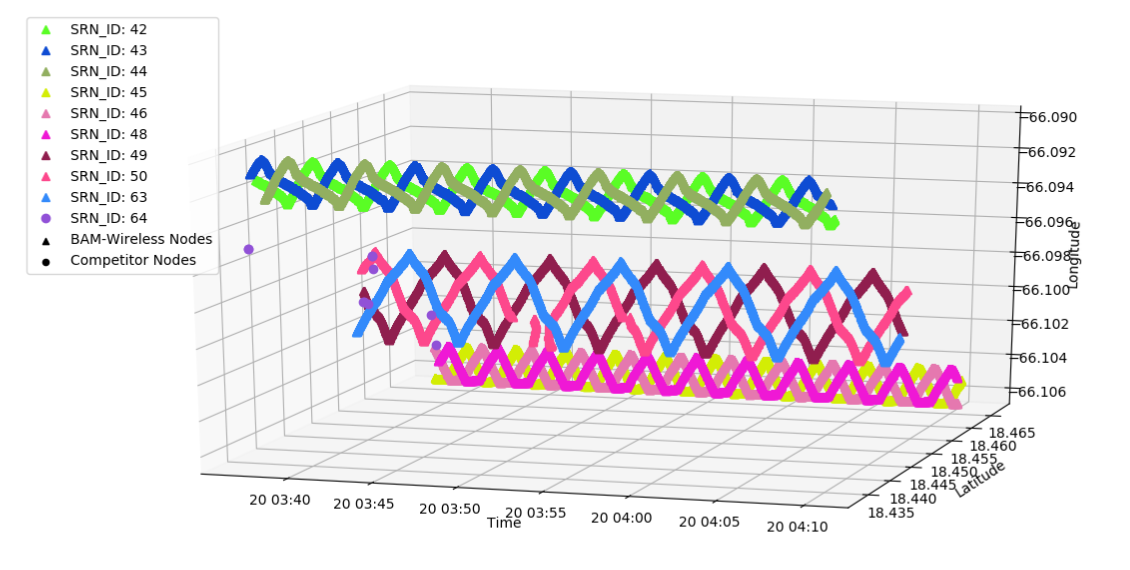
\includegraphics[width = 1.0\textwidth]{Payline_Node_GPS_Locations.PNG}
    \caption{A $3$-D visualization of the node movements during the DARPA SC$2$ Payline scenario}
    \label{fig:1}
\end{figure}

\begin{figure}
    \centering
    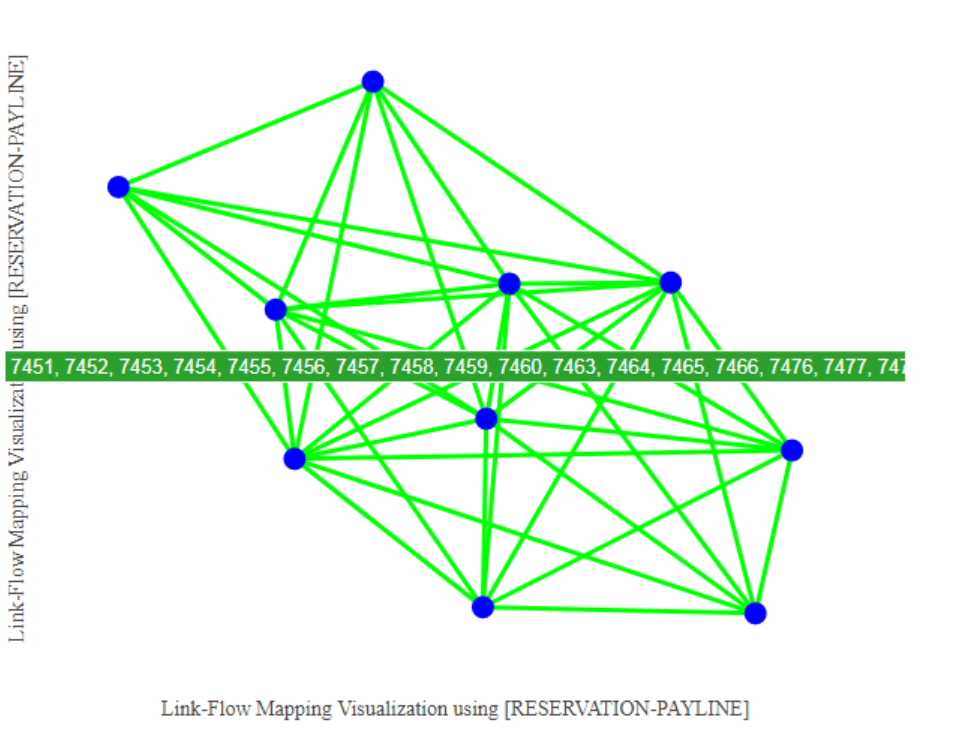
\includegraphics[width = 1.0\textwidth]{Network_Graph_Payline.PNG}
    \caption{A graph of network links within our Purdue BAM! Wireless radio network, during the DARPA SC$2$ Payline scenario}
    \label{fig:2}
\end{figure}

\begin{figure}
    \centering
    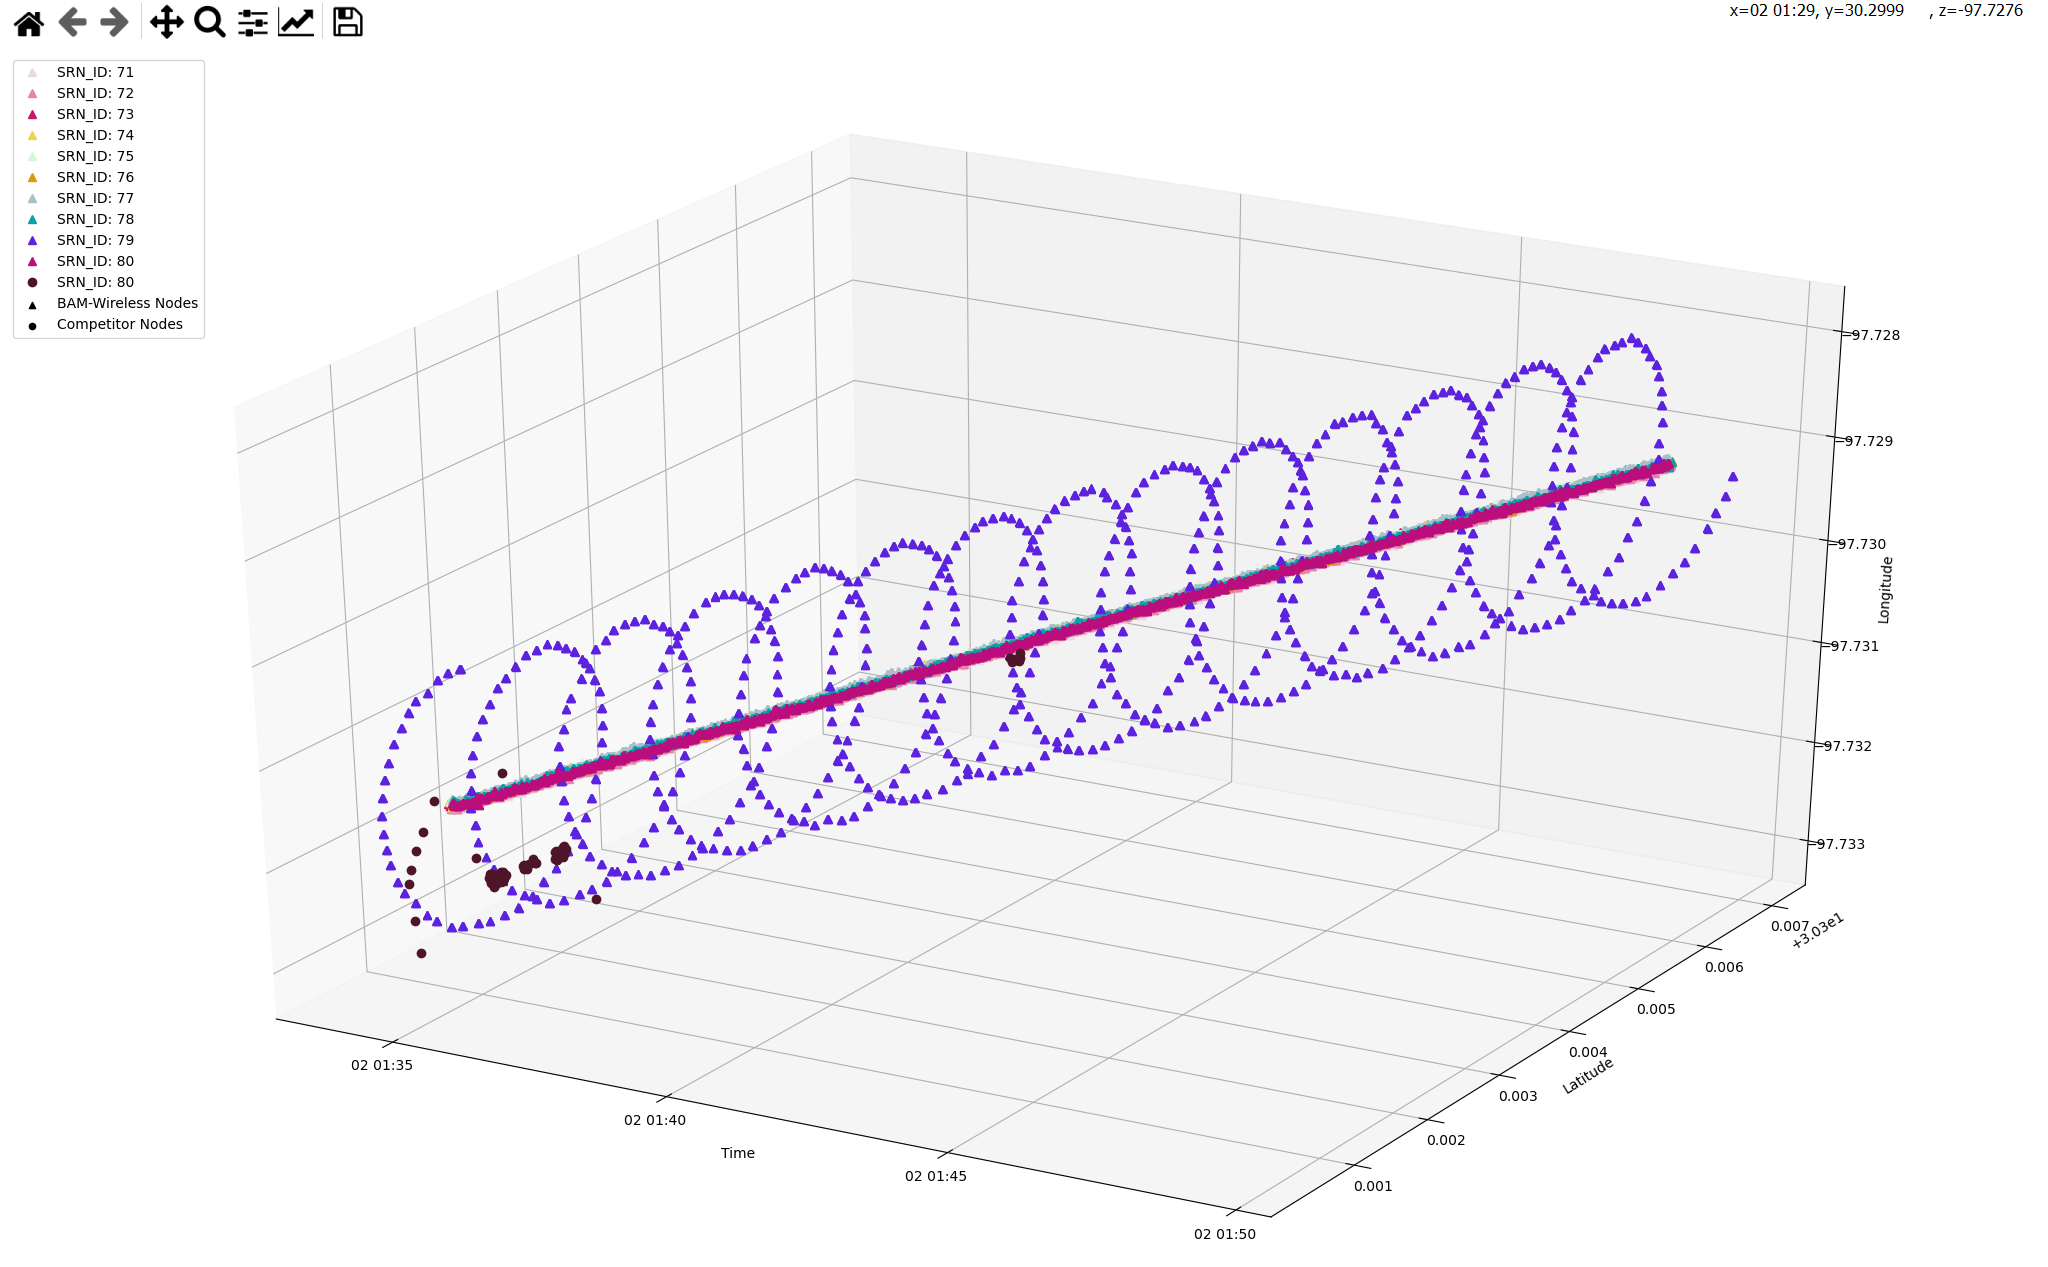
\includegraphics[width = 1.0\textwidth]{Alleys_GPS.PNG}
    \caption{A $3$-D visualization of the node movements during the DARPA SC$2$ Alleys of Austin scenario}
    \label{fig:3}
\end{figure}

\begin{figure}
    \centering
    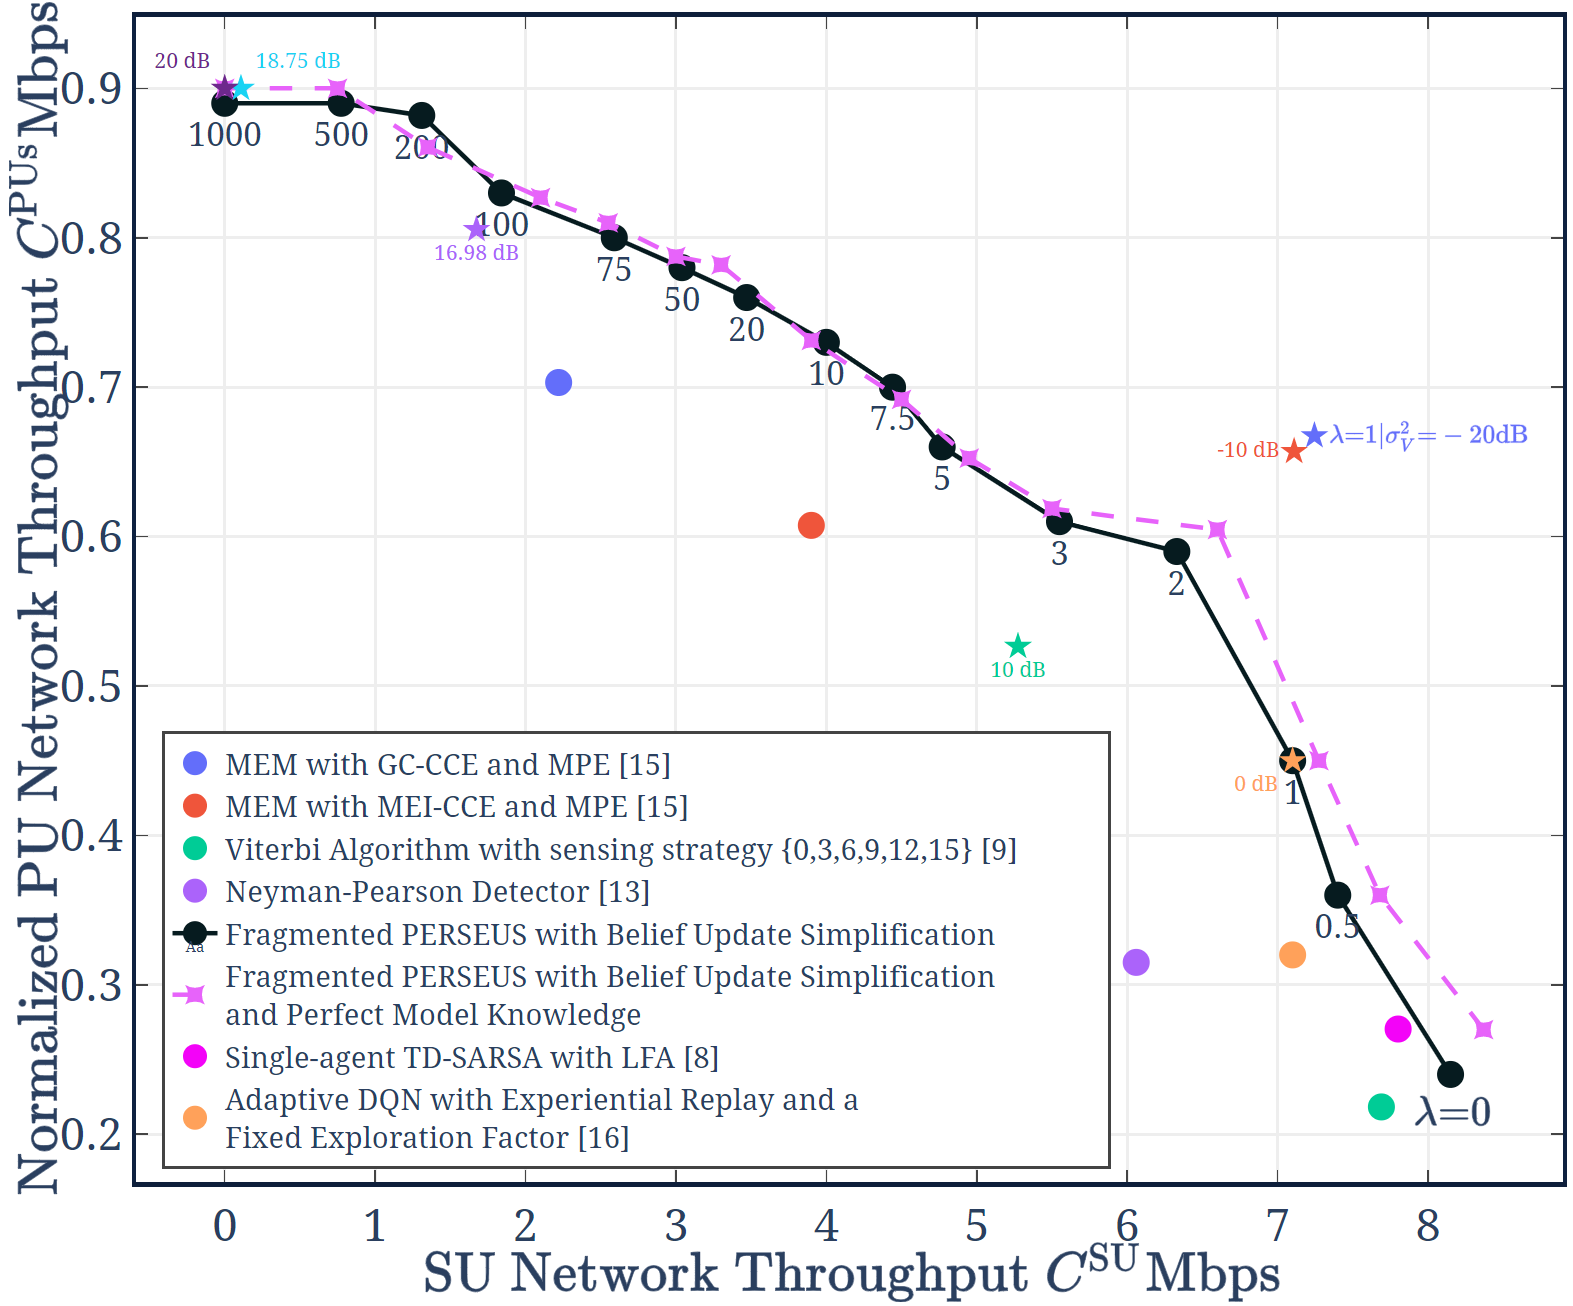
\includegraphics[width = 1.0\textwidth]{Evaluation_2.png}
    \caption{``Normalized PU(s) Throughput" v ``SU Network Throughput" under varying noise power levels (at the SU receiver) for our framework ($\lambda{=}1$) -- in addition to penalty-based tuning and state-of-the-art comparisons}
    \label{fig:4}
\end{figure}

\end{document}
